    \documentclass{beamer}
    \usepackage{siunitx}
    \usepackage{tfrupee}
    \let\vec\mathbf
    \mode<presentation>
    \usepackage{amsmath}
    \usepackage{amssymb}
    %\usepackage{advdate}
    \usepackage{adjustbox}
    %\usepackage{subcaption}
    \usepackage{enumitem}
    \usepackage{multicol}
    \usepackage{mathtools}
    \usepackage{listings}
    \usepackage{url}
    \usetheme{Boadilla}
    \usecolortheme{lily}
    \setbeamertemplate{footline}
    {
      \leavevmode%
      \hbox{%
      \begin{beamercolorbox}[wd=\paperwidth,ht=2.25ex,dp=1ex,right]{author in head/foot}%
        \insertframenumber{} / \inserttotalframenumber\hspace*{2ex} 
      \end{beamercolorbox}}%
      \vskip0pt%
    }
    \setbeamertemplate{navigation symbols}{}
    \providecommand{\nCr}[2]{\,^{#1}C_{#2}} % nCr
    \providecommand{\nPr}[2]{\,^{#1}P_{#2}} % nPr
    \providecommand{\mbf}{\mathbf}
    \providecommand{\pr}[1]{\ensuremath{\Pr\left(#1\right)}}
    \providecommand{\qfunc}[1]{\ensuremath{Q\left(#1\right)}}
    \providecommand{\sbrak}[1]{\ensuremath{{}\left[#1\right]}}
    \providecommand{\lsbrak}[1]{\ensuremath{{}\left[#1\right.}}
    \providecommand{\rsbrak}[1]{\ensuremath{{}\left.#1\right]}}
    \providecommand{\brak}[1]{\ensuremath{\left(#1\right)}}
    \providecommand{\lbrak}[1]{\ensuremath{\left(#1\right.}}
    \providecommand{\rbrak}[1]{\ensuremath{\left.#1\right)}}
    \providecommand{\cbrak}[1]{\ensuremath{\left\{#1\right\}}}
    \providecommand{\lcbrak}[1]{\ensuremath{\left\{#1\right.}}
    \providecommand{\rcbrak}[1]{\ensuremath{\left.#1\right\}}}
    \theoremstyle{remark}
    \newtheorem{rem}{Remark}
    \newcommand{\sgn}{\mathop{\mathrm{sgn}}}
    
    \providecommand{\res}[1]{\Res\displaylimits_{#1}} 
    \providecommand{\norm}[1]{\left\lVert#1\right\rVert}
    \providecommand{\mtx}[1]{\mathbf{#1}}
    \providecommand{\abs}[1]{\left\vert#1\right\vert}
    \providecommand{\fourier}{\overset{\mathcal{F}}{ \rightleftharpoons}}
    %\providecommand{\hilbert}{\overset{\mathcal{H}}{ \rightleftharpoons}}
    \providecommand{\system}{\overset{\mathcal{H}}{ \longleftrightarrow}}
    	%\newcommand{\solution}[2]{\textbf{Solution:}{#1}}
    %\newcommand{\solution}{\noindent \textbf{Solution: }}align
    \providecommand{\dec}[2]{\ensuremath{\overset{#1}{\underset{#2}{\gtrless}}}}
    \newcommand{\myvec}[1]{\ensuremath{\begin{pmatrix}#1\end{pmatrix}}}
    
    \title{Matrices in Geometry - 10.5.5}
    \author{EE25BTECH11037  Divyansh}
    \date{Sept, 2025}
    
    \begin{document}
    
    \maketitle
    
    
    \section{Problem}
    \begin{frame}
    \frametitle{Problem Statement}
    Construct a tangent to a circle of radius $4cm$ from a point on the concentric circle of radius $6cm$ and measure its length. Also verify the measurement by actual calculation.
    \end{frame}
    
    \section{Solution}
    \begin{frame}{Solution}
    Let center be the origin. Then the circle with radius $4 \ cm$ is
\begin{align}
    \vec{C} \ : \ \vec{x}^{\top}\vec{V}\vec{x} + 2\vec{u}^{\top}\vec{x} + f=0 \ ; \ \vec{V}=\myvec{1&0\\0&1} \ , \ \vec{u}=\myvec{0\\0} \ , \ f=-16
\end{align}
Let the external point from which the tangent is drawn be $\vec{h}=\myvec{6\\0}$.
    \end{frame}
    
    \begin{frame}{Solution}
    Let us calculate the matrix $\Sigma$
\begin{align}
    \Sigma=\brak{\vec{V}\vec{h} + \vec{u}}\brak{\vec{V}\vec{h} + \vec{u}}^{\top} - g\brak{\vec{h}}\vec{V}\\
    g\brak{\vec{h}}=\vec{h}^{\top}\vec{V}\vec{h} + 2\vec{u}^{\top}\vec{h} + f =\norm{\vec{h}}^2 +f =36-16 =20\\
    \Sigma = \vec{h}\vec{h}^{\top} - g\brak{\vec{h}}\vec{V}=\myvec{6 \\ 0}\myvec{6 & 0} - 20\myvec{ 1& 0 \\ 0 &1}\\
    \implies \Sigma=\myvec{16 & 0 \\ 0 & -20}
\end{align}
The eigenvalues of the matrix $\Sigma$ are clearly $\lambda_1=16$ and $\lambda_2=-20$
    \end{frame}

    \begin{frame}{Solution}
        The normalized eigenvectors form the matrix $\vec{P}$.
\begin{align}
    \vec{P}=\myvec{1 & 0\\0&1}
\end{align}
The direction vectors of the two tangents are
\begin{align}
    \vec{m}=\vec{P}\myvec{\abs{\lambda_2} \\ \pm\sqrt{\abs{\lambda_1}}}=\myvec{2\sqrt{5} \\ \pm 4}
\end{align}
    \end{frame}
    \begin{frame}{Solution}
        The length of the tangent is given by
\begin{align}
    \norm{\vec{T}-\vec{h}}=\abs{\mu} \norm{\vec{m}} \ , \ \brak{\text{$\mu$ is a parameter}}\\
    \mu= -\dfrac{\vec{m}^{\top} \brak{\vec{V}\vec{h} + \vec{u}}}{\norm{\vec{m}}^2} =-\dfrac{\myvec{2\sqrt{5} & 4} \myvec{6\\0}}{\norm{\myvec{2\sqrt{5} \\ 4}}^2}=-\dfrac{\sqrt{5}}{3}\\
    \therefore \norm{\vec{T}-\vec{h}}=\dfrac{\sqrt{5}}{3} \times 6 = 2\sqrt{5} \approx 4.47 \ cm
\end{align}
From the figure given below, we can verify that both lengths are equal and equal to $4.47$ cm.
    \end{frame}
    \begin{frame}{Solution}
    
    \begin{figure}
    \centering
    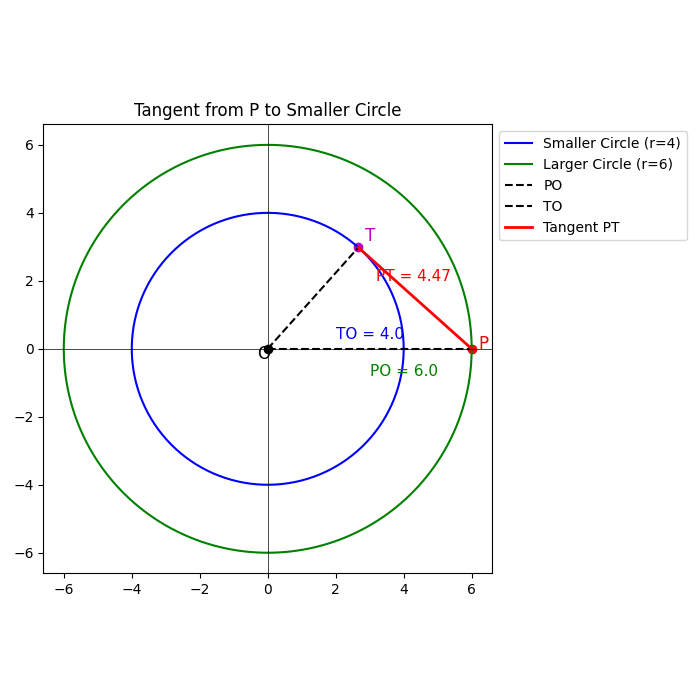
\includegraphics[width=0.6\columnwidth]{figs/1.png}
    \caption{Graph for 10.5.5}
    \label{fig:placeholder}
\end{figure}
    \end{frame}
    
    
    \end{document}